\documentclass[a4paper,10pt]{article}
\usepackage[margin=18mm,footskip=9mm]{geometry}
\usepackage{iftex}
\ifPDFTeX
  \usepackage[T1]{fontenc}
  \usepackage[utf8]{inputenc}
  \usepackage[scaled=0.96]{helvet}
  \renewcommand{\familydefault}{\sfdefault}
\else
  \usepackage{fontspec}
  \setmainfont{texgyreheros}[Extension=.otf,
    UprightFont=*-regular, BoldFont=*-bold,
    ItalicFont=*-italic, BoldItalicFont=*-bolditalic]
\fi
\newif\ifChineseMemo
\ChineseMemotrue
\ifChineseMemo
  \ifPDFTeX
    \PackageError{finance-memo}{Chinese text requires XeLaTeX or LuaLaTeX}{}
  \else
    \usepackage[UTF8,fontset=fandol]{ctex}
    \renewcommand{\familydefault}{\sfdefault}
  \fi
\fi
\usepackage{booktabs,graphicx,xcolor,caption,xurl,fancyhdr,array}
\definecolor{MemoBlue}{HTML}{203E70}
\definecolor{MemoRule}{HTML}{B9C8DF}
\usepackage[colorlinks=true,linkcolor=MemoBlue,urlcolor=MemoBlue]{hyperref}
\captionsetup{font=small,labelfont=bf,skip=4pt}
\setlength{\parindent}{0pt}
\setlength{\parskip}{5pt}
\renewcommand{\arraystretch}{1.16}
\pagestyle{fancy}
\fancyhf{}
\renewcommand{\headrulewidth}{0pt}
\renewcommand{\footrulewidth}{0.3pt}

\newcommand{\ReportTitle}{五家大型科技公司同业对比}
\newcommand{\ReportType}{同业研究简报}
\newcommand{\ReportDate}{2026年10月31日}
\newcommand{\DataDate}{2026年10月26日}
\newcommand{\ReportScope}{最近完整财年｜金额单位：十亿美元｜比率单位：\%}
\newcommand{\TeamName}{同业研究}
\newcommand{\DeskName}{财务比较}
\newcommand{\Coverage}{苹果、微软、Alphabet、亚马逊、英伟达}
\newcommand{\KeyFinding}{英伟达净利率为55.6\%，居五家之首；亚马逊营收规模最高，但净利率为10.8\%。}
\fancyfoot[L]{\scriptsize\TeamName}
\fancyfoot[R]{\scriptsize\ReportType}

\begin{document}
\begin{minipage}[t]{0.70\textwidth}
\vspace{0pt}
{\small\ReportDate}\par\medskip
{\color{MemoBlue}\hrule height 0.5pt}\smallskip
{\large\ReportType}\par
{\LARGE\bfseries\ReportTitle}\par\medskip
\ReportScope
\end{minipage}\hfill
\begin{minipage}[t]{0.23\textwidth}
\vspace{0pt}\raggedleft
\colorbox{MemoBlue}{\parbox[c][19mm][c]{0.86\linewidth}{\centering\color{white}\bfseries\TeamName}}\par\medskip
\DeskName
\end{minipage}
\par\bigskip
{\color{MemoBlue}\hrule height 0.5pt}\medskip
{\large\KeyFinding}\par\bigskip

\begin{minipage}[t]{0.58\textwidth}
\vspace{0pt}\raggedright
\setlength{\parskip}{4pt}
\textbf{范围与读者}\par
本报告供需要快速比较经营规模和盈利能力的研究读者参考，覆盖苹果、微软、Alphabet、亚马逊和英伟达。财务数据取自各公司最近一个营收、经营利润和净利润齐备的完整财年。净利率为净利润除以同期营收。

\textbf{主要发现}\par
亚马逊营收为716.9十亿美元，规模居五家之首；英伟达营收同比增长65.5\%，增速最快。按净利率从高到低排列，依次为英伟达55.6\%、微软40.3\%、Alphabet 32.8\%、苹果26.9\%和亚马逊10.8\%。

\textbf{解释}\par
营收规模高，并不意味着净利率也高。这些比较仅反映历史年度差异，不能据此推断商业模式与财务表现之间的因果关系，也不构成估值或投资建议。

\textbf{风险与限制}\par
五家公司财年截止日不同，不能将数据视为同一自然期间。GAAP净利润可能受投资损益和一次性税项影响；毛利润一部分来自直接披露，另一部分按同期间营收减成本计算。
\end{minipage}\hfill
\begin{minipage}[t]{0.38\textwidth}
\vspace{0pt}\small
\captionof{figure}{净利率对比}\label{fig:net-margin}
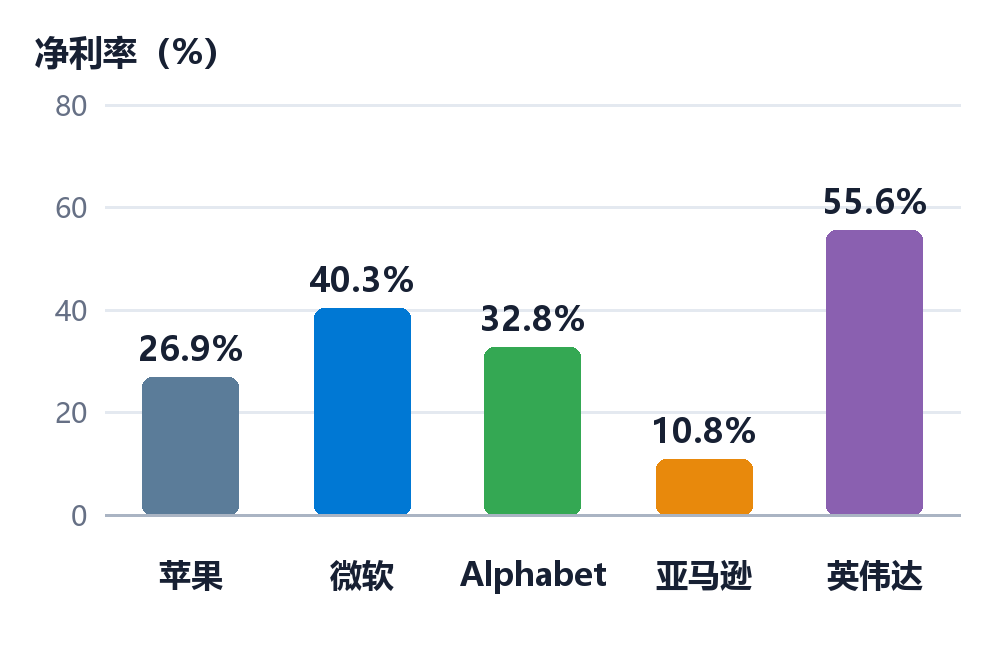
\includegraphics[width=\linewidth]{../output/figures/net_margin_report.png}
{\scriptsize 注：净利率＝净利润÷同期营收。各公司财年截止日见表\ref{tab:peer-comparison}，财年期间不同。\par}
{\scriptsize 来源：SEC EDGAR XBRL company facts API；按\texttt{comparison.json}绘制。\par}

\end{minipage}
\par\medskip
\captionof{table}{五家公司年度财务对比}\label{tab:peer-comparison}
{\scriptsize 金额单位：十亿美元；比率单位：\%；均保留一位小数。各公司财年截止日见表内，财年期间不同。\par}
{\footnotesize\setlength{\tabcolsep}{5pt}\begin{tabular}{l c r r r r r}
\toprule
公司 & 财年截止日 & 营收 & 营收同比 & 毛利率 & 经营利润率 & 净利率 \\
\midrule
苹果 & 2025-09-27 & 416.2 & 6.4\% & 46.9\% & 32.0\% & 26.9\% \\
微软 & 2026-06-30 & 331.8 & 17.8\% & 67.9\% & 46.8\% & 40.3\% \\
Alphabet & 2025-12-31 & 402.8 & 15.1\% & 59.7\% & 32.0\% & 32.8\% \\
亚马逊 & 2025-12-31 & 716.9 & 12.4\% & 50.3\% & 11.2\% & 10.8\% \\
英伟达 & 2026-01-25 & 215.9 & 65.5\% & 71.1\% & 60.4\% & 55.6\% \\
\bottomrule
\end{tabular}
\par}
{\scriptsize 注：营收同比按相邻完整财年计算。毛利润优先采用同期间披露值；未直接披露时，以同期间营收减营业成本计算。\par}
{\scriptsize 来源：SEC EDGAR XBRL company facts API；五家公司营收均已通过10-K独立核对。\par}

\par\vfill

{\color{MemoRule}\hrule height 0.4pt}\medskip
\begin{minipage}[t]{0.34\textwidth}
\vspace{0pt}\small
\textbf{覆盖范围}\par\Coverage
\end{minipage}\hfill
\begin{minipage}[t]{0.62\textwidth}
\vspace{0pt}\footnotesize
\setlength{\parskip}{3pt}
\textbf{来源与日期。}财务数据取自\texttt{comparison.json}，原始来源为SEC EDGAR XBRL company facts API，数据文件生成于\DataDate；10-K仅用于独立核对，核对记录见\texttt{verification.md}。

\textbf{核验。}五家公司营收均已与对应10-K合并利润表核对，数值、单位和期间一致（5/5）。表格和图形均由脚本根据同一JSON生成，增长率和利润率已经复算。

\textbf{编制方法。}表格文件仅包含\texttt{tabular}，图形文件仅保留坐标、柱形和数值；图题、表题、来源及财年注释在\texttt{report/sections/}中的包装文件内单独维护。
\end{minipage}
\end{document}
